% restart.png: a run that stopped, and its restart. Make it in this folder with, for any scratch folder T:
%   pdflatex -output-directory=T fig_restart.tex
%   python3 pdf_to_png.py T/fig_restart.pdf ../restart.png
\documentclass[11pt,tikz,border=1.5pt]{standalone}
% Shared preamble of all figures. Every fig_*.tex is compiled on its own, see the comment at its top; the fonts are those of the matplotlib
% style xzc_sans (amsmath, amssymb, amsfonts, sfmath), so that line drawings and data plots look the same.
\usepackage{amsmath,amssymb,amsfonts}
\usepackage{sfmath}
\renewcommand{\familydefault}{\sfdefault}
\usepackage{graphicx}
\usetikzlibrary{arrows.meta,calc,positioning,decorations.pathreplacing,backgrounds,shapes.geometric}
% species: Al gray, Mg orange, Zn blue; red marks the vacancy and the jumping atom
\definecolor{cAl}{HTML}{B8BCC2}
\definecolor{cMg}{HTML}{E08A2E}
\definecolor{cZn}{HTML}{3F78B5}
\definecolor{cOne}{HTML}{C8423B}
\definecolor{cTwo}{HTML}{3F78B5}
\definecolor{cThree}{HTML}{3E9B5C}
\definecolor{cFour}{HTML}{E0A21B}
\definecolor{cGray}{HTML}{7E858F}
\definecolor{cDark}{HTML}{2B2B2B}
\newcommand{\panel}[1]{\textbf{(#1)}}
\newcommand{\DM}{D_{\mathrm{MEP}}}
\newcommand{\KI}{K_{\mathrm{I}}}
\newcommand{\KF}{K_{\mathrm{F}}}
\newcommand{\dE}{\Delta E}
\newcommand{\Ea}{\Delta E_{\mathrm{a}}}
\newcommand{\ea}{\Delta e_{\mathrm{a}}}
\newcommand{\Ebind}{E_{\mathrm{bind}}^{\mathrm{site}}}
% a ball with a soft highlight, like the rendered spheres
\makeatletter
\pgfdeclareradialshading[tikz@ball]{softball}{\pgfpoint{-9bp}{9bp}}{%
  color(0bp)=(tikz@ball!22!white); color(6bp)=(tikz@ball!62!white); color(13bp)=(tikz@ball!96!white);
  color(20bp)=(tikz@ball!92!black); color(27bp)=(tikz@ball!74!black); color(50bp)=(tikz@ball!55!black)}
\makeatother
\tikzset{
  every picture/.append style={line cap=round, line join=round},
  every node/.append style={font=\small},
  img/.style={inner sep=0pt, anchor=south west},
  lab/.style={font=\normalsize, inner sep=1pt, anchor=north west},
  above lab/.style={font=\normalsize, inner sep=1pt, anchor=south west},
  capt/.style={align=center, anchor=north},
  atom/.style={circle, ball color=#1, shading=softball, minimum size=12pt, inner sep=0pt},
  atom/.default=cAl,
  vac/.style={circle, draw=cOne, line width=1.1pt, fill=white, minimum size=11.5pt, inner sep=0pt},
  arr/.style={-{Stealth[length=5pt]}, line width=0.8pt},
  dbl/.style={{Stealth[length=4pt]}-{Stealth[length=4pt]}, line width=0.8pt},
  jump/.style={arr, cOne, line width=1.2pt},
  block/.style={-{Triangle[length=8pt, width=13pt]}, line width=5pt, cTwo!38},
  cell axis/.style={-{Triangle[length=6pt, width=5.5pt]}, line width=1.2pt, black},
  dir/.style={fill=white, fill opacity=0.75, text opacity=1, font=\footnotesize, inner sep=1.5pt},
}
\graphicspath{{img/}}
% data plots are included at one scale: \plot{name}{x}{y}{file}
\newcommand{\plotscale}{0.6}
\newcommand{\plot}[4]{\node[img] (#1) at (#2,#3) {\includegraphics[scale=\plotscale]{#4}};}
\newcommand{\plotlabel}[2]{\node[above lab] at ($(#1.north west)+(-0.05,0.02)$) {\panel{#2}};}
% legend of the species, first entry at (#1,#2): Al, Mg, Zn (and the vacancy)
\tikzset{leg/.style={anchor=base west, inner sep=2pt, yshift=-3.2pt}}
\newcommand{\specieslegend}[2]{%
  \foreach \lx/\lc/\lt in {0/cAl/Al, 1.2/cMg/Mg, 2.4/cZn/Zn} {
    \node[atom=\lc, minimum size=10pt] at ({#1+\lx},#2) {}; \node[leg] at ({#1+\lx+0.2},#2) {\lt};}}
\newcommand{\vacancylegend}[2]{\node[vac, minimum size=9.5pt] at (#1,#2) {}; \node[leg] at ({#1+0.2},#2) {vacancy};}

\newcommand{\file}[1]{{\footnotesize\ttfamily\detokenize{#1}}}
\begin{document}
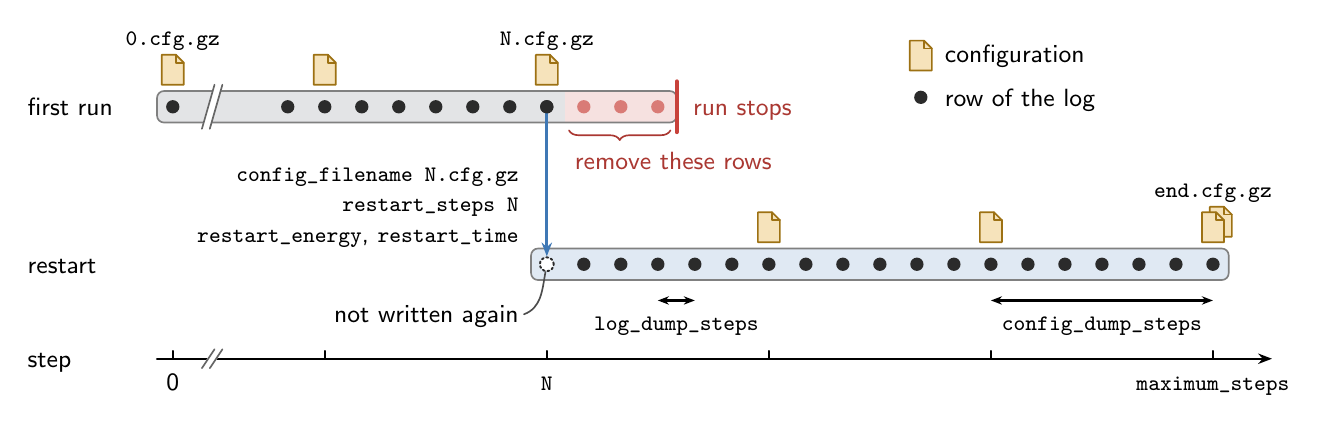
\begin{tikzpicture}[
    bar/.style={black!50, line width=0.6pt, rounded corners=2.5pt},
    row/.style={circle, fill=cDark, minimum size=4.8pt, inner sep=0pt},
    norow/.style={circle, draw=cDark, densely dotted, line width=0.7pt, fill=white, minimum size=5pt, inner sep=0pt},
    lbl/.style={inner sep=1.5pt, anchor=base},
    side/.style={anchor=base west, inner sep=0pt, yshift=-3.2pt},
    tick/.style={line width=0.6pt},
    sheet/.style={draw=cFour!70!black, fill=cFour!30, line width=0.6pt}]
  % x of step 0, of step N, and of the stop; config_dump_steps and log_dump_steps
  \def\xo{1.85}\def\xN{6.60}\def\xs{8.25}\def\dc{2.82}\def\dl{0.47}
  % a configuration: a sheet with a folded corner
  \newcommand{\sheet}[2]{%
    \begin{scope}[shift={(#1,#2)}]
      \filldraw[sheet] (-0.14,0) -- (-0.14,0.38) -- (0.04,0.38) -- (0.14,0.28) -- (0.14,0) -- cycle;
      \draw[sheet, fill=none] (0.04,0.38) -- (0.04,0.28) -- (0.14,0.28);
    \end{scope}}
  \newcommand{\cut}[3]{% a cut through a bar or an axis at x = #1 from y = #2 to #3
    \draw[white, line width=3pt, line cap=butt] (#1-0.08,#2) -- (#1+0.08,#3);
    \draw[black!60, line width=0.6pt] (#1-0.13,#2) -- (#1+0.03,#3) (#1-0.03,#2) -- (#1+0.13,#3);}
  % ---------------- first run ----------------
  \begin{scope}
    \clip[rounded corners=2.5pt] (\xo-0.2,1.5) rectangle (\xs,1.9);
    \fill[cGray!22] (\xo-0.2,1.5) rectangle (\xN+0.5*\dl,1.9);
    \fill[cOne!16] (\xN+0.5*\dl,1.5) rectangle (\xs,1.9);
  \end{scope}
  \draw[bar] (\xo-0.2,1.5) rectangle (\xs,1.9);
  \cut{\xo+0.5}{1.42}{1.98}
  \node[row] at (\xo,1.7) {};
  \foreach \k in {-7,...,0} \node[row] at (\xN+\k*\dl,1.7) {};
  \foreach \k in {1,2,3} \node[row, fill=cOne!70] at (\xN+\k*\dl,1.7) {};
  \foreach \x in {\xo,\xN-\dc,\xN} {\sheet{\x}{1.98}}
  \node[lbl] at (\xo,2.48) {\file{0.cfg.gz}};
  \node[lbl] at (\xN,2.48) {\file{N.cfg.gz}};
  \node[side] at (0,1.7) {first run};
  \draw[cOne, line width=1.6pt] (\xs,1.38) -- (\xs,2.02);
  \node[side, text=cOne!85!black] at (\xs+0.2,1.7) {run stops};
  \draw[decorate, decoration={brace, mirror, amplitude=3.5pt}, line width=0.6pt, cOne!85!black]
    (\xN+0.6*\dl,1.4) -- (\xs-0.08,1.4);
  \node[anchor=north west, inner sep=0pt, text=cOne!85!black] at (\xN+0.35,1.13) {remove these rows};
  % ---------------- restart ----------------
  \draw[bar, fill=cTwo!16] (\xN-0.2,-0.5) rectangle (\xN+3*\dc+0.2,-0.1);
  \node[norow] (again) at (\xN,-0.3) {};
  \foreach \k in {1,...,18} \node[row] at (\xN+\k*\dl,-0.3) {};
  \sheet{\xN+\dc}{-0.02} \sheet{\xN+2*\dc}{-0.02} \sheet{\xN+3*\dc+0.1}{0.05} \sheet{\xN+3*\dc}{-0.02}
  \node[lbl] at (\xN+3*\dc,0.55) {\file{end.cfg.gz}};
  \node[side] at (0,-0.3) {restart};
  \draw[arr, cTwo, line width=1pt] (\xN,1.62) -- (\xN,-0.2);
  \node[row] at (\xN,1.7) {};
  \node[anchor=east, align=right, inner sep=0pt] at (\xN-0.35,0.42)
    {\file{config_filename N.cfg.gz}\\ \file{restart_steps N}\\ \file{restart_energy}, \file{restart_time}};
  \node[anchor=base east, inner sep=0pt, yshift=-3.2pt] (note) at (\xN-0.35,-0.93) {not written again};
  \draw[black!70, line width=0.6pt] ($(note.east)+(0.06,0.03)$) to[out=20, in=-100] (again);
  \draw[dbl] (\xN+3*\dl,-0.76) -- (\xN+4*\dl,-0.76); \node[lbl] at (\xN+3.5*\dl,-1.14) {\file{log_dump_steps}};
  \draw[dbl] (\xN+2*\dc,-0.76) -- (\xN+3*\dc,-0.76); \node[lbl] at (\xN+2.5*\dc,-1.14) {\file{config_dump_steps}};
  % ---------------- axis of the steps ----------------
  \draw[arr] (\xo-0.2,-1.5) -- (\xN+3*\dc+0.75,-1.5);
  \cut{\xo+0.5}{-1.62}{-1.38}
  \foreach \x in {\xo,\xN-\dc,\xN,\xN+\dc,\xN+2*\dc,\xN+3*\dc} \draw[tick] (\x,-1.5) -- ++(0,0.1);
  \node[lbl] at (\xo,-1.9) {0};
  \node[lbl] at (\xN,-1.9) {\file{N}};
  \node[lbl] at (\xN+3*\dc,-1.9) {\file{maximum_steps}};
  \node[side] at (0,-1.5) {step};
  % ---------------- legend ----------------
  \sheet{11.35}{2.16} \node[anchor=base west, inner sep=0pt] at (11.65,2.26) {configuration};
  \node[row] at (11.35,1.82) {}; \node[side] at (11.65,1.82) {row of the log};
\end{tikzpicture}
\end{document}
